\section{Introdução}\label{introduuxe7uxe3o}

Para a prática 3 será necessário montar um circuito que irá realizar
comunicação serial com equipamento externo, no caso o PIC18F4550 na
plataforma SanUSB comunicando-se com um ESP8266.

\section{Objetivo}\label{objetivo}

Enviar um valor inteiro para o ESP8266 através de uma URL para que o
ESP8266 identifique o valor e envie através de porta serial o valor para
o PIC18F4550 fazendo com que ele interrompa e inicie o processo de
alternar LEDs para um sinal de pedestres e automóveis.

\section{Comunicação}\label{comunicauxe7uxe3o}

Ao receber uma requisição HTTP, com uma URL do tipo
\texttt{http://172.24.2.95/?val=10}, o ESP8266 obtém o seguinte
\emph{payload}:

\begin{verbatim}
GET /?val=10 HTTP/1.1
Host: 172.24.2.95
Accept-Language: en-US,en;q=0.5
Accept-Encoding: gzip, deflate
Connection: keep-alive
Upgrade-Insecure-Requests: 1
\end{verbatim}

Logo na primeira linha está o valor que desejamos enviar ao PIC.

Abaixo um trecho do codigo fonte (Linguagem Lua):

\begin{Shaded}
\begin{Highlighting}[]
\CommentTok{-- a simple http server}
\KeywordTok{srv} \OtherTok{=} \KeywordTok{net}\OtherTok{.}\NormalTok{createServer}\OtherTok{(}\KeywordTok{net}\OtherTok{.}\KeywordTok{TCP}\OtherTok{)}
\KeywordTok{srv}\NormalTok{:listen}\OtherTok{(}\DecValTok{80}\OtherTok{,} \KeywordTok{function}\OtherTok{(}\KeywordTok{conn}\OtherTok{)}
    \KeywordTok{conn}\NormalTok{:on}\OtherTok{(}\StringTok{"receive"}\OtherTok{,} \KeywordTok{function}\OtherTok{(}\KeywordTok{sck}\OtherTok{,} \KeywordTok{payload}\OtherTok{)}
        \KeywordTok{if} \KeywordTok{string}\OtherTok{.}\NormalTok{match}\OtherTok{(}\KeywordTok{payload}\OtherTok{,} \StringTok{"val="}\OtherTok{)} \KeywordTok{then}
            \KeywordTok{tempo} \OtherTok{=} \KeywordTok{string}\OtherTok{.}\NormalTok{match}\OtherTok{(}\KeywordTok{payload}\OtherTok{,} \StringTok{'%d+'}\OtherTok{)}
            \FunctionTok{print}\OtherTok{(}\KeywordTok{tempo}\OtherTok{)}
        \KeywordTok{end}
        
        \KeywordTok{sck}\NormalTok{:send}\OtherTok{(}\StringTok{"HTTP/1.0 200 OK}\OtherTok{\textbackslash{}r\textbackslash{}n}\StringTok{"}
            \OtherTok{..} \StringTok{"Content-Type: text/html}\OtherTok{\textbackslash{}r\textbackslash{}n\textbackslash{}r\textbackslash{}n}\StringTok{<h1>"}
            \OtherTok{..} \StringTok{"Iniciando semáforo com tempo de "}
            \OtherTok{..} \KeywordTok{tempo}
            \OtherTok{..} \StringTok{" segundos<br>Transmitido via ESP8266</h1>"}\OtherTok{)}
    \KeywordTok{end}\OtherTok{)}
\KeywordTok{end}\OtherTok{)}
\end{Highlighting}
\end{Shaded}

A ideia é que quando o payload conter a String \texttt{val=} (linha 5),
então o tempo é obtido através do \emph{regex} (Regular Expression)
\texttt{\%d+}, indicando que é um valor inteiro, um dígito ou mais
(linha 6). Finalmente o ESP envia o valor para a porta serial (linha 7)
através de um \texttt{print}.

\section{Circuito}\label{circuito}

As Figuras \ref{fig:circuito1}, \ref{fig:circuito2} e
\ref{fig:circuito3} mostram a evolução do circuito.

\begin{figure}[h]
    \centering
    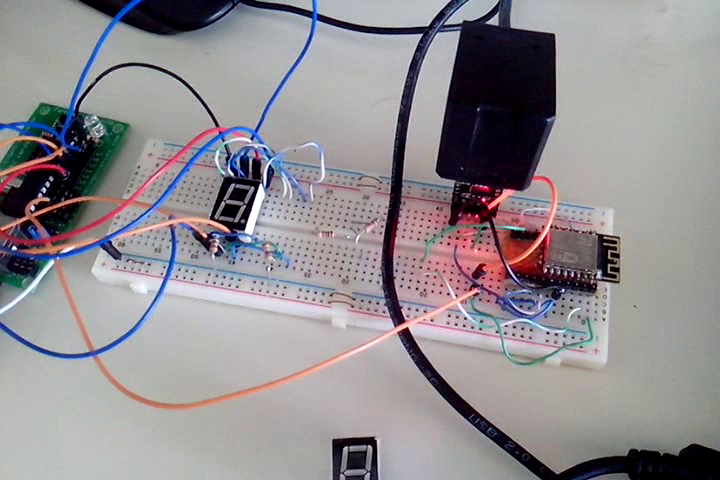
\includegraphics[scale=0.5]{img/vlcsnap-2016-10-20-16h24m17s640.png}
    \caption{Montagem Inicial apenas com 1 display de 7 segmentos}\label{fig:circuito1}
\end{figure}

\begin{figure}[h]
    \centering
    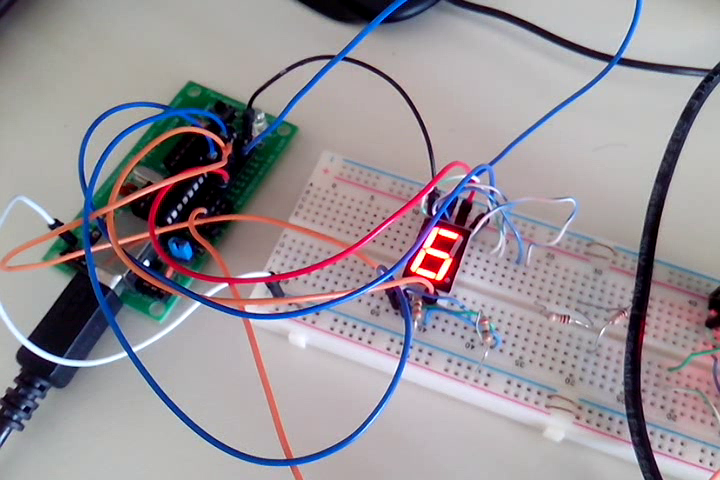
\includegraphics[scale=0.5]{img/vlcsnap-2016-10-20-16h24m03s183.png}
    \caption{Envio de comando apenas para ligar, ainda sem indicar valor}\label{fig:circuito2}
\end{figure}

\begin{figure}[h]
    \centering
    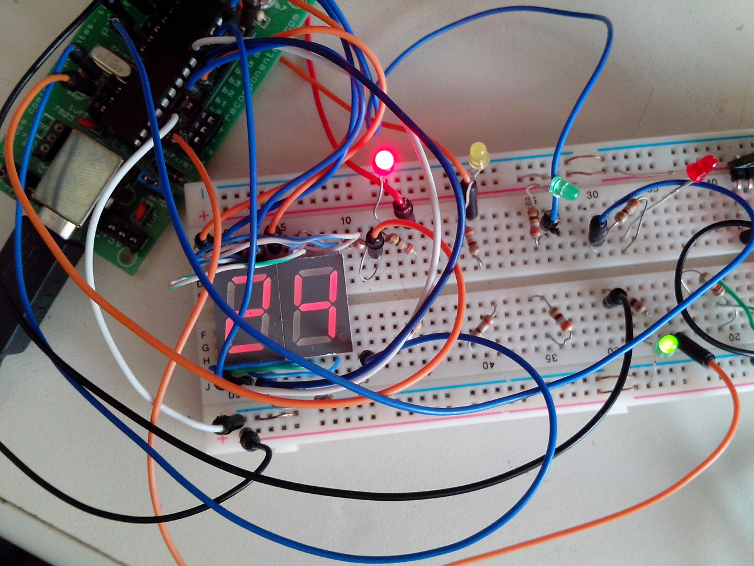
\includegraphics[scale=0.5]{img/IMG_20161006_103716.jpg}
    \caption{Circuito Final, com semáforo e valor passado via porta serial com 2 displays de 7 segmentos}\label{fig:circuito3}
\end{figure}

\section{Recepção serial}\label{recepuxe7uxe3o-serial}

Para receber o valor pela serial foi usado a opção de verificar se houve
interrupção e ler o valor da porta serial. Abaixo um trecho do código:

\begin{Shaded}
\begin{Highlighting}[]
\DataTypeTok{char} \NormalTok{char_byte;}
\DataTypeTok{char} \NormalTok{comando[}\DecValTok{2}\NormalTok{];}
\DataTypeTok{int} \NormalTok{pos = }\DecValTok{0}\NormalTok{;}
\DataTypeTok{int} \NormalTok{valor_recebido = }\DecValTok{0}\NormalTok{;}
\DataTypeTok{void} \NormalTok{interrupt interrupcao() \{}
    \KeywordTok{if} \NormalTok{(serial_interrompeu) \{}
        \NormalTok{serial_interrompeu = }\DecValTok{0}\NormalTok{;}
        \NormalTok{char_byte = ReadUSART();}
        \CommentTok{// recebe bytes até '\textbackslash{}n'}
        \KeywordTok{if} \NormalTok{(char_byte != }\CharTok{'\textbackslash{}n'}\NormalTok{) \{}
            \NormalTok{comando[pos] = char_byte;}
            \NormalTok{pos++;}
        \NormalTok{\} }\KeywordTok{else} \NormalTok{\{}
            \NormalTok{valor_recebido = }\DecValTok{1}\NormalTok{;}
            \NormalTok{pos = }\DecValTok{0}\NormalTok{;}
        \NormalTok{\}}
    \NormalTok{\}}
\NormalTok{\}}
\end{Highlighting}
\end{Shaded}

